\chapter{声母}\label{charonset}

\section{辅音音位}

米亚罗话共有33个辅音音位，如表\ref{consonant}所示。

\begin{table}[H]
\vspace{5pt}
    \centering
    \caption{辅音音位}
    \label{consonant}
\begin{tabular}{cccccccc}
    
   \toprule
     & & 双唇 & 齿龈 & 龈后 & 龈-腭 & 硬腭 & 软腭 \\
   \midrule
   爆发音 & 清不送气 & /p/ & /t/ &  & & & /k/ \\
    & 清送气 & /pʰ/ & /tʰ/ &  & & & /kʰ/ \\
    & 浊不送气 & /b/ & /d/ &  & & & /ɡ/ \\
    鼻音 & & /m/ & /n/ &  & & /ɲ/ & /ŋ/ \\
    擦音 & 清 &  & /s/ & /ʃ/ & /ɕ/ & & /x/ \\
     & 浊 &  & /z/ & /ʒ/ & & &  \\
    塞擦音 & 清不送气 &  & /ts/ & /tʃ/ & /tɕ/ & &  \\
    & 清送气 &  & /tsʰ/ & /tʃʰ/ & /tɕʰ/ & &  \\
    & 浊不送气 & & /dz/ & /dʒ/ & /dʑ/ & &  \\
    颤音 & &  & /r/ &  &  & &  \\
    边擦音 & &  & /ɬ/ &  &  & &  \\
    边近音 & &  & /l/ &  &  & &  \\
    近音 & & /w/ &  &  &  & /j/ &  \\
   \bottomrule
\end{tabular}
\end{table}

表\ref{conex}列出了全部的单辅音声母示例。

\begin{table}[H]
\vspace{5pt}
    \centering
    \caption{辅音示例}
    \label{conex}
\begin{tabular}{ccc|ccc}
     \toprule
	/p/ & [kɐ-po] & “纺” & /l/ & [kə-lə] & “重的” \\
	/pʰ/ & [kɐ-pʰô] & “躲” & /ɬ/ & [ɬɐ̂] & “神” \\
	/b/ & [kə-bə̂s] & “灰暗的” & /ʃ/ & [kə-ʃək] & “新的” \\
	/m/ & [tɐ-mî] & “脚” & /tʃ/ & [kə-tʃən] & “短的” \\
	/w/ & [tə-wom] & “尸体” & /tʃʰ/ & [kɐ-tʃʰət] & “插” \\
	/t/ & [kɐ-tɐ̂] & “脱” & /dʒ/ & [tə-dʒɿ̂] & “皮肤” \\ 
	/tʰ/ & [tə-tʰɐ̂] & “书” & /ɕ/ & [tɐ-ɕet] & “梳子” \\ 
	/d/ & [tɐ-dok] & “毒药” & /tɕ/ & [kɐ-tɕet] & “关门” \\ 
	/n/ & [tə-nə] & “乳房” & /tɕʰ/ & [kɐ-tɕʰî] & “去” \\
	/s/ & [kɐ-sɐ̂r] & “娶” & /dʑ/ & [kʰə-dʑe] & “石杆菜（紫花碎米芥）” \\ 
	/z/ & [tə-zɐ̂] & “饭” & /ɲ/ & [ɲo] & “你们” \\ 
	/ts/ & [kə-tsə̂r] & “咸” & /j/ & [kɐ-jok] & “仰头” \\ 
	/tsʰ/ & [kə-tsʰɐr] & “闪光的” & /k/ & [tɐ-ku] & “头” \\ 
	/dz/ & [tə-mdzu] & “刺” & /kʰ/ & [kɐ-kʰo] & “晒” \\ 
	/r/ & [rowû] & “石头” & /ɡ/ & [tɐ-ɡɐm] & “蛋” \\ 
	/ʒ/ & [ʒowu] & “棉花” & /ŋ/ & [ŋos] & “是” \\ 
    /x/ & [kə-xɐw] & “好” &   &   &   \\
   \bottomrule
\end{tabular}
\end{table}

\subsection{爆发音}

米亚罗话的爆发音有清不送气、清送气、浊不送气三分对立，发声部位有双唇、齿龈、软腭。表\ref{ploex}列出了爆发音在元音/a/上的近似最小对。

\begin{table}[H]
\vspace{5pt}
    \centering
    \caption{爆发音的准最小对}
    \label{ploex}
\begin{tabular}{ccc}
   \toprule
    音位 & 例子 & 释义 \\
   \midrule
   /p/ & [tɐ-\textbf{pɐ̂}] & “父亲”  \\
   /pʰ/ & [\textbf{pʰɐ}tɐk] & “面条”  \\
   /b/ & [\textbf{bɐ}lə̂] & “没有角的牦牛”  \\
   /t/ & [kɐ-\textbf{tɐ̂}] & “放置”  \\
   /tʰ/ & [tə-\textbf{tʰɐ̂}] & “书”  \\
   /d/ & [tɐ-\textbf{dɐ}ste] & “火葬场”  \\
   /k/ & [\textbf{kɐ}-] & “动词词典形前缀” \\
   /kʰ/ & [\textbf{kʰɐ}lə̂] & “风” \\
   /ɡ/ & [tɐ-\textbf{ɡɐ}m] & “蛋” \\
   \bottomrule
\end{tabular}
\end{table}

其中齿龈爆发音/t/、/tʰ/、/d/在实际语音实现上更接近齿音[t̪]、[t̪ʰ]、[d̪]。

很多研究证明，爆发音的清浊对立不一定完全来自于发声起始时间（VOT）显示的带声性\cite{cho2019voice}；但通过测量米亚罗话的爆发音VOT，可以认为米亚罗话的清浊对立呈现出较为纯粹的带声性对立，见图\ref{votb}至\ref{votkh}，图中红线表示爆破释放，蓝线表示起声；浊不送气爆发音若在释放前已经出现周期性振动，则记为负值。测量结果见表\ref{plosivevot}。

\begin{figure}[H]
\centering
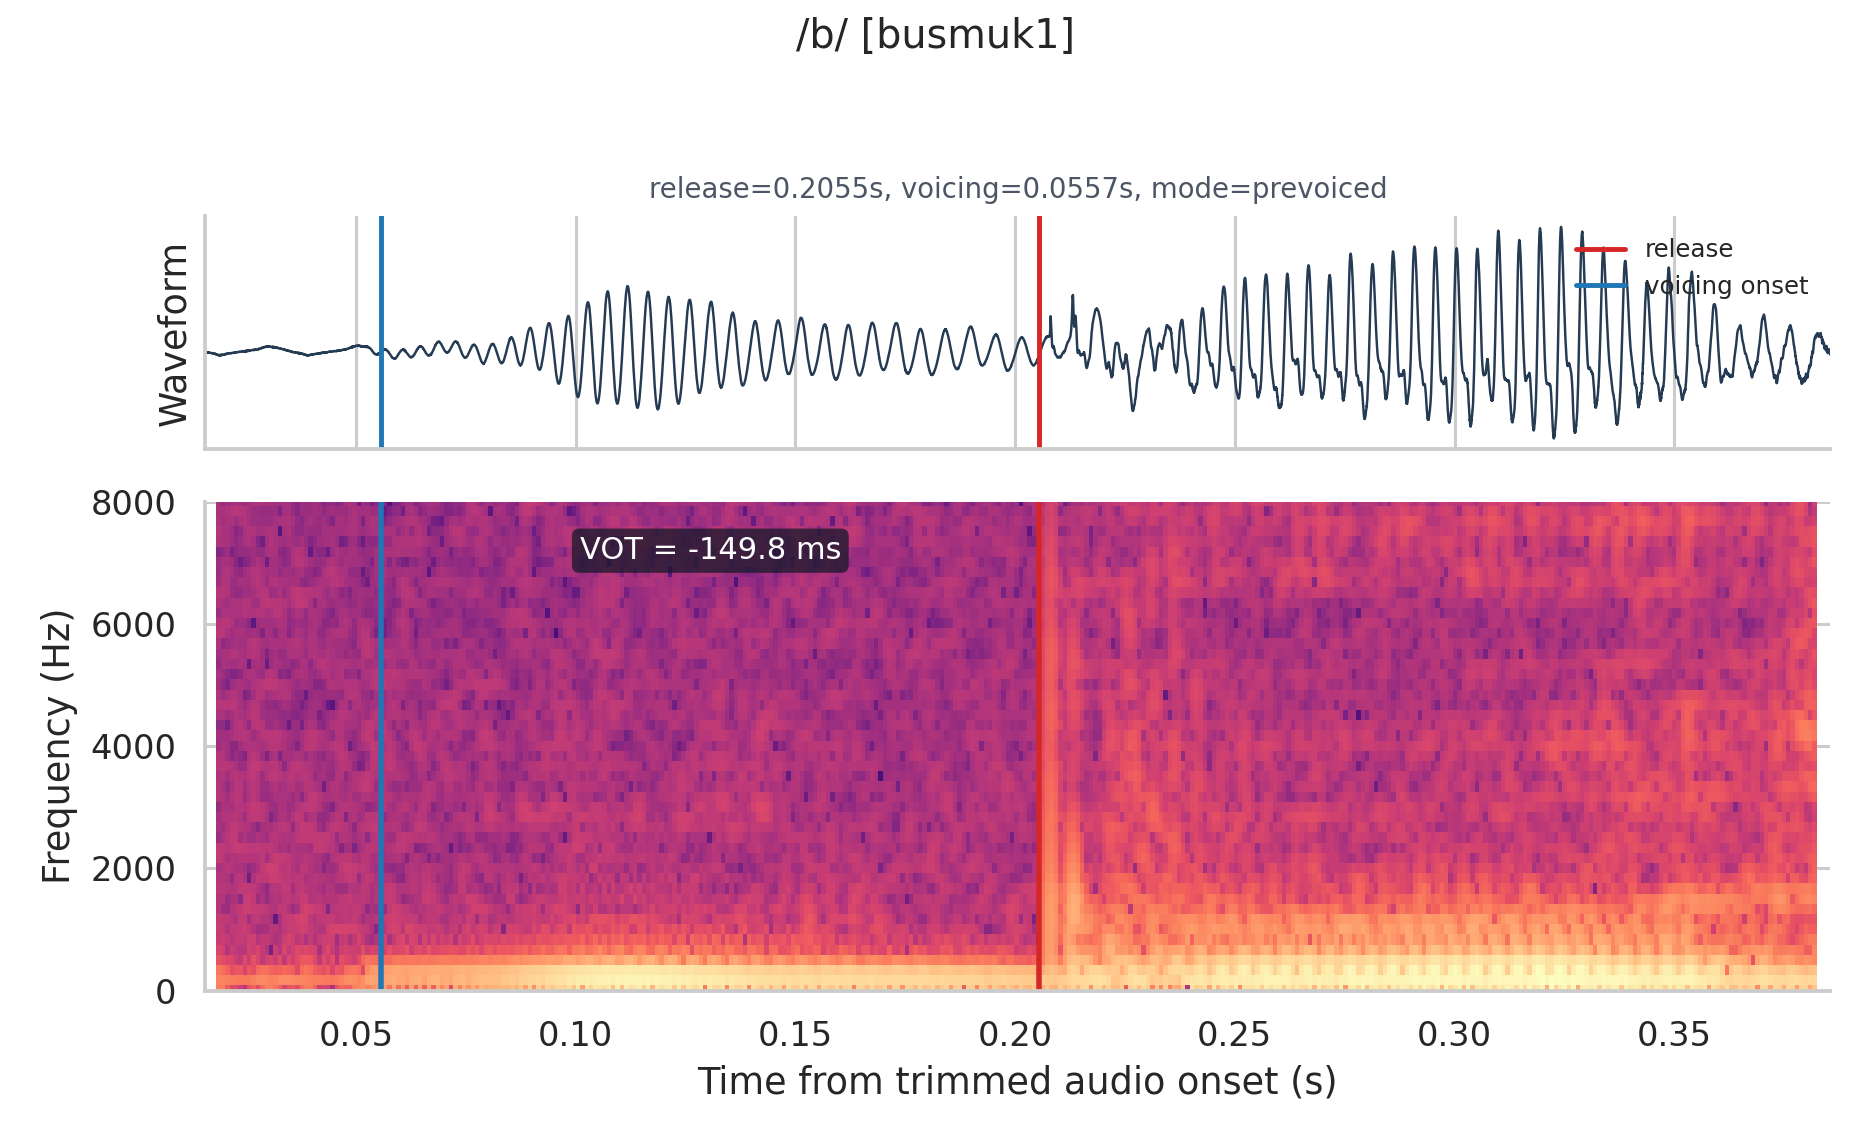
\includegraphics[width=0.8\textwidth]{img/vot_b.png}
\caption{[busmuk]“发霉”的发声起始时间}
\label{votb}
\end{figure}

\begin{figure}[H]
\centering
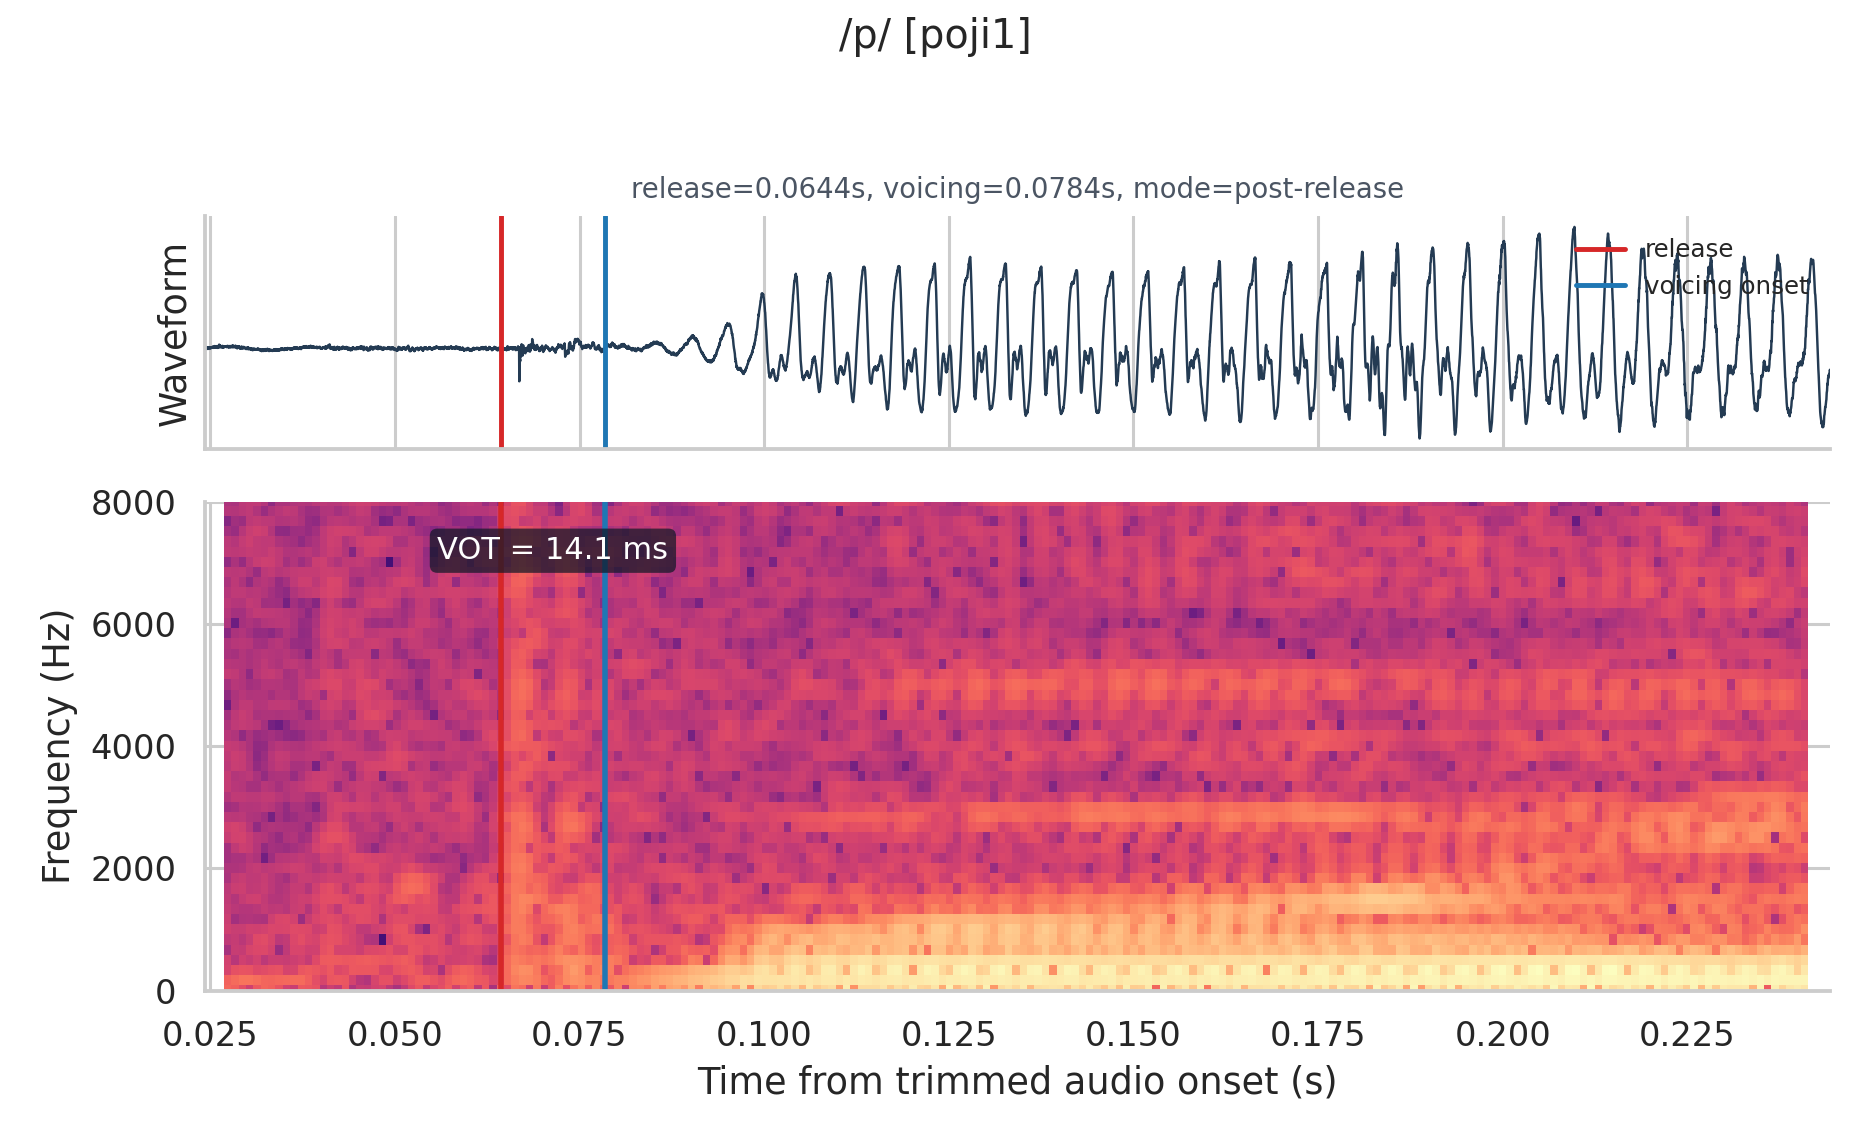
\includegraphics[width=0.8\textwidth]{img/vot_p.png}
\caption{[poji]“老鼠”的发声起始时间}
\label{votp}
\end{figure}

\begin{figure}[H]
\centering
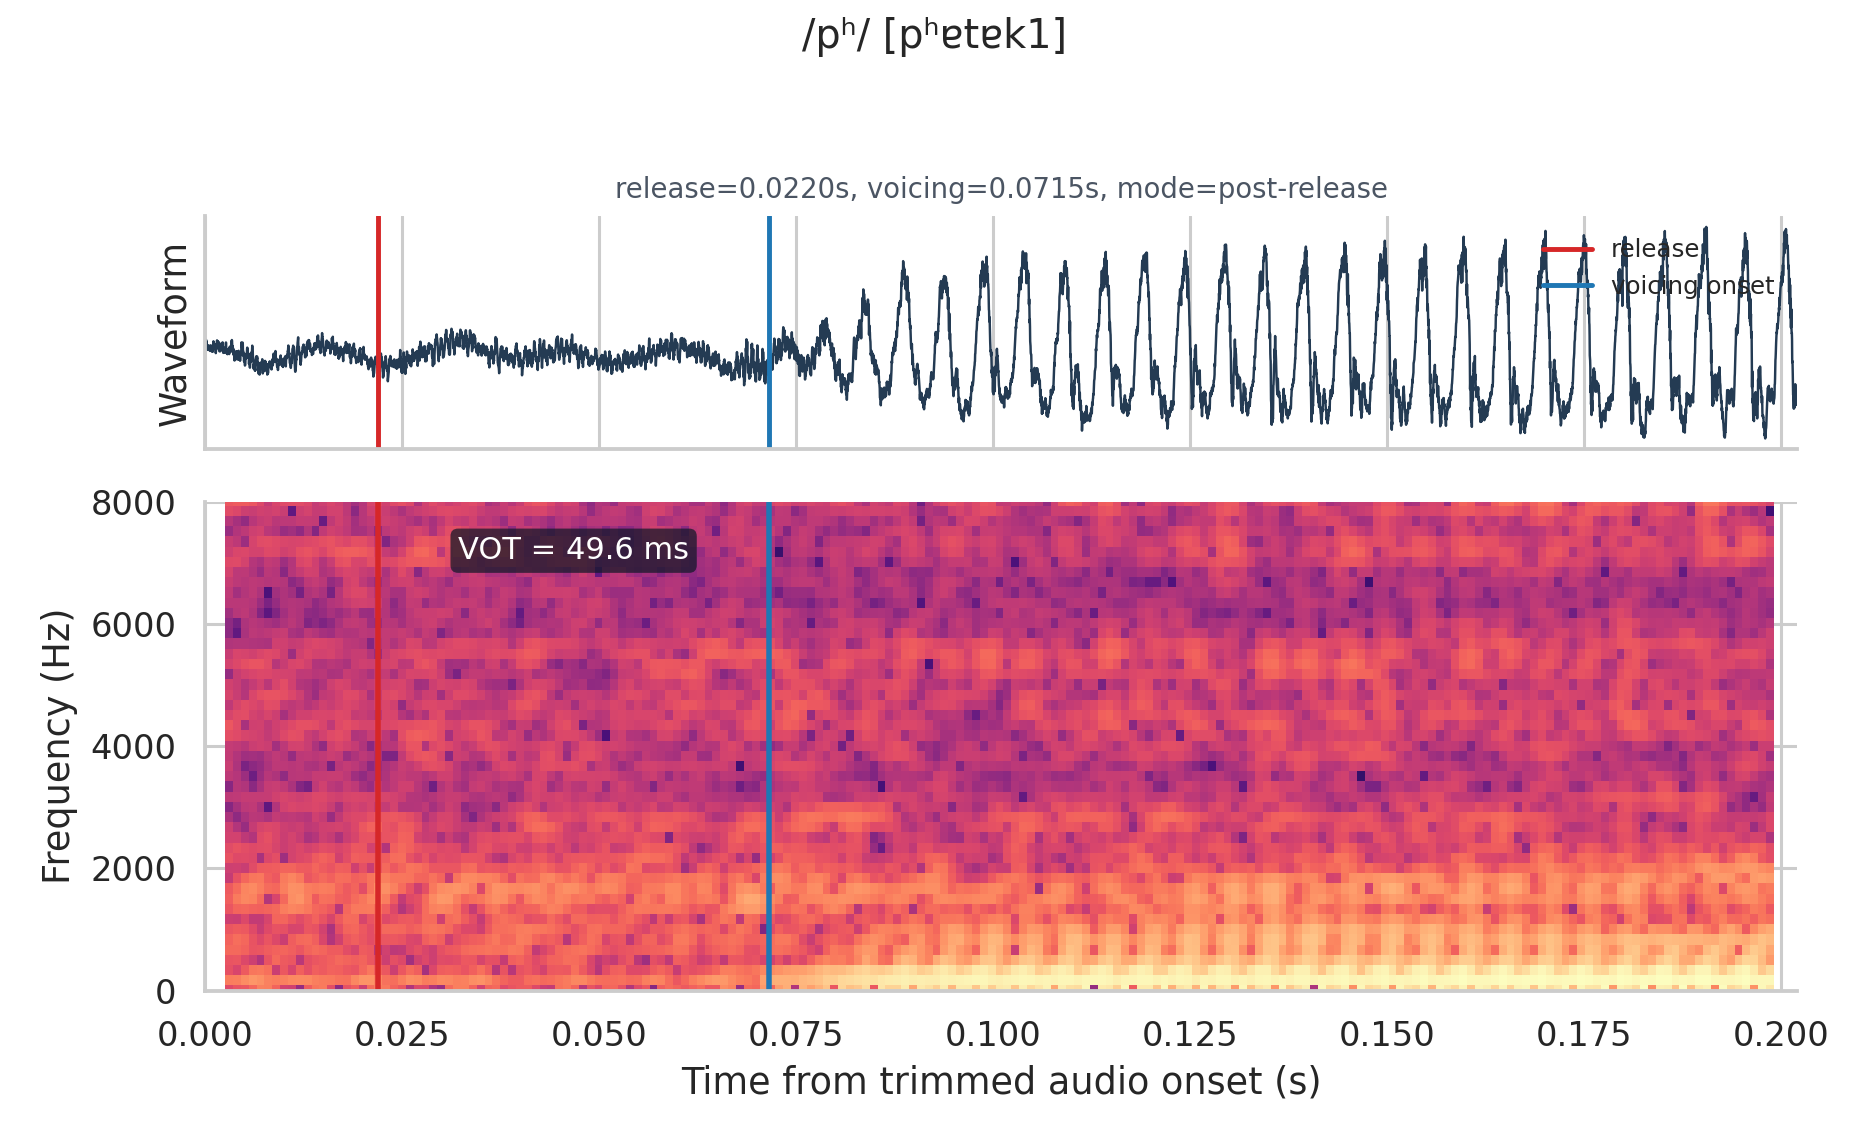
\includegraphics[width=0.8\textwidth]{img/vot_ph.png}
\caption{[pʰɐtɐk]“面条”的发声起始时间}
\label{votph}
\end{figure}

\begin{figure}[H]
\centering
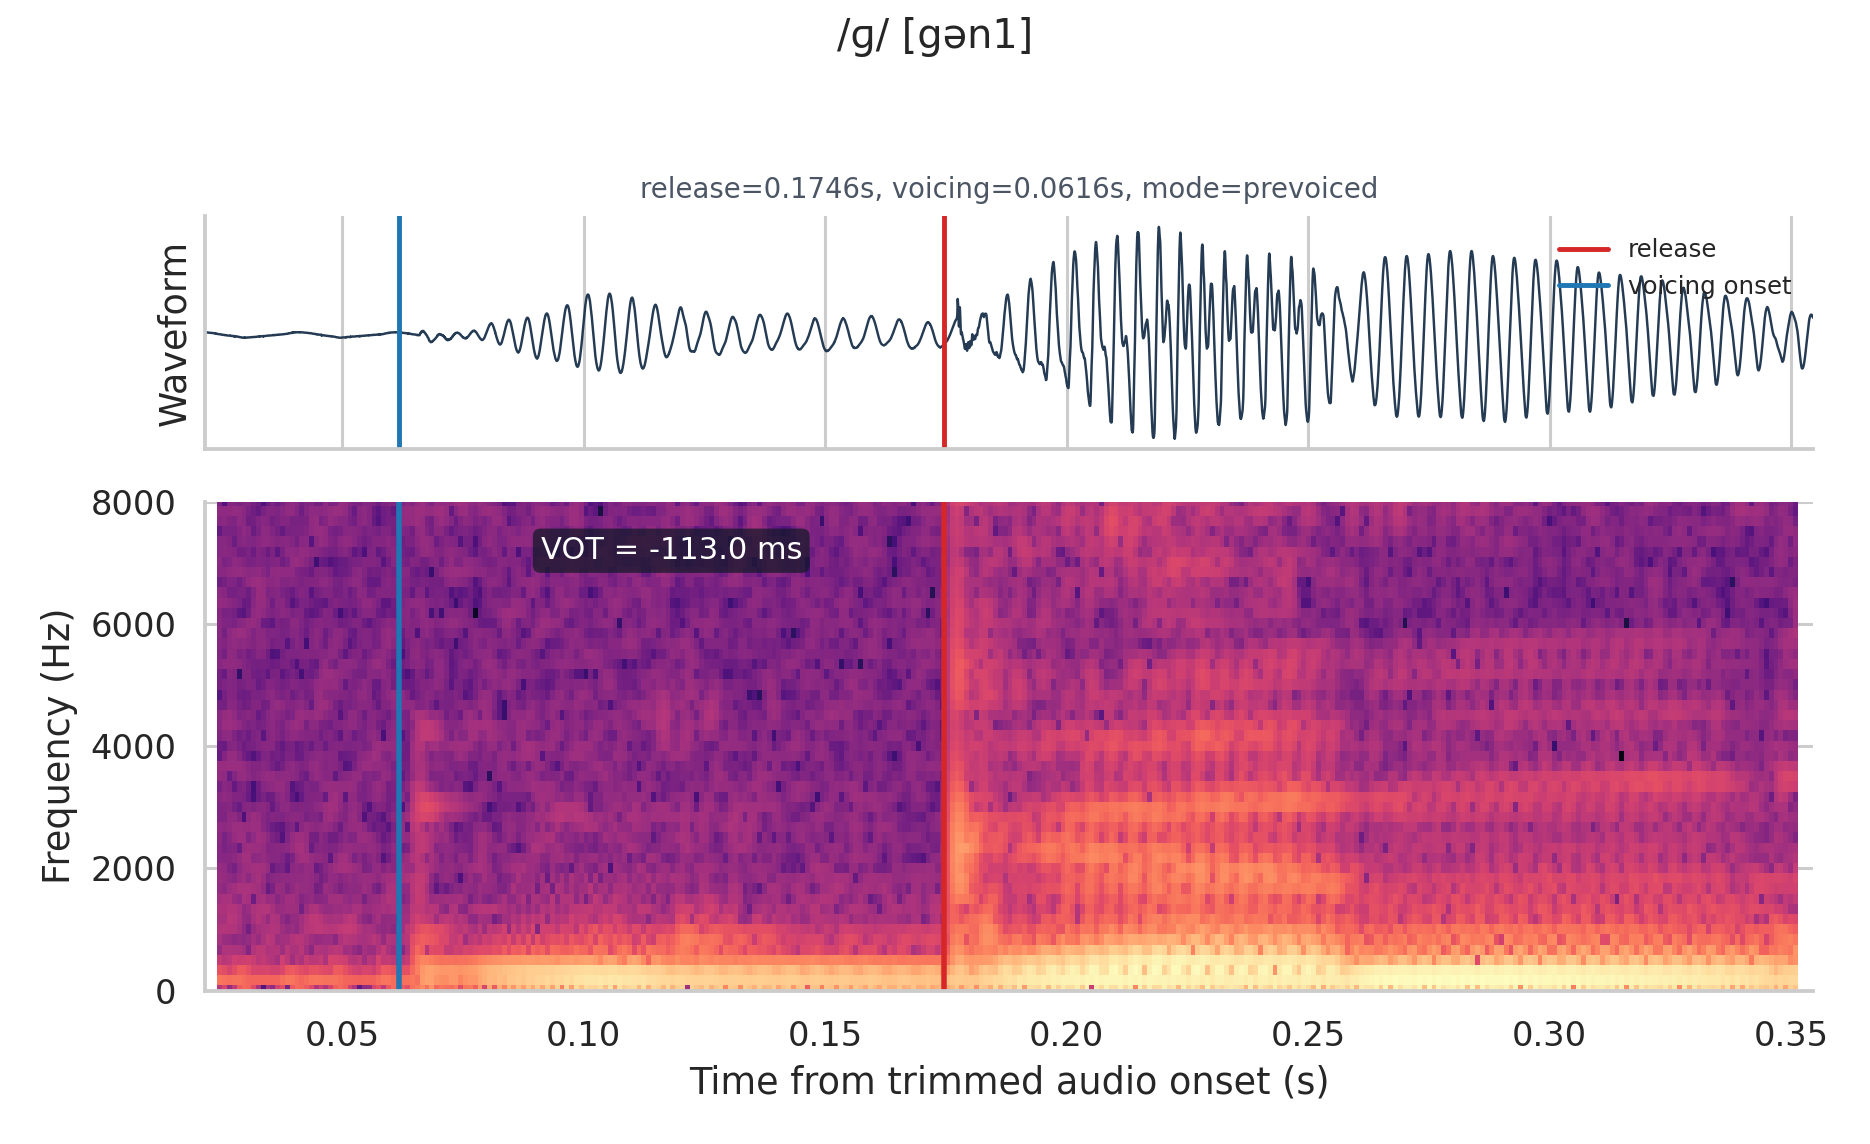
\includegraphics[width=0.8\textwidth]{img/vot_g.png}
\caption{[ɡən]“很”的发声起始时间}
\label{votg}
\end{figure}

\begin{figure}[H]
\centering
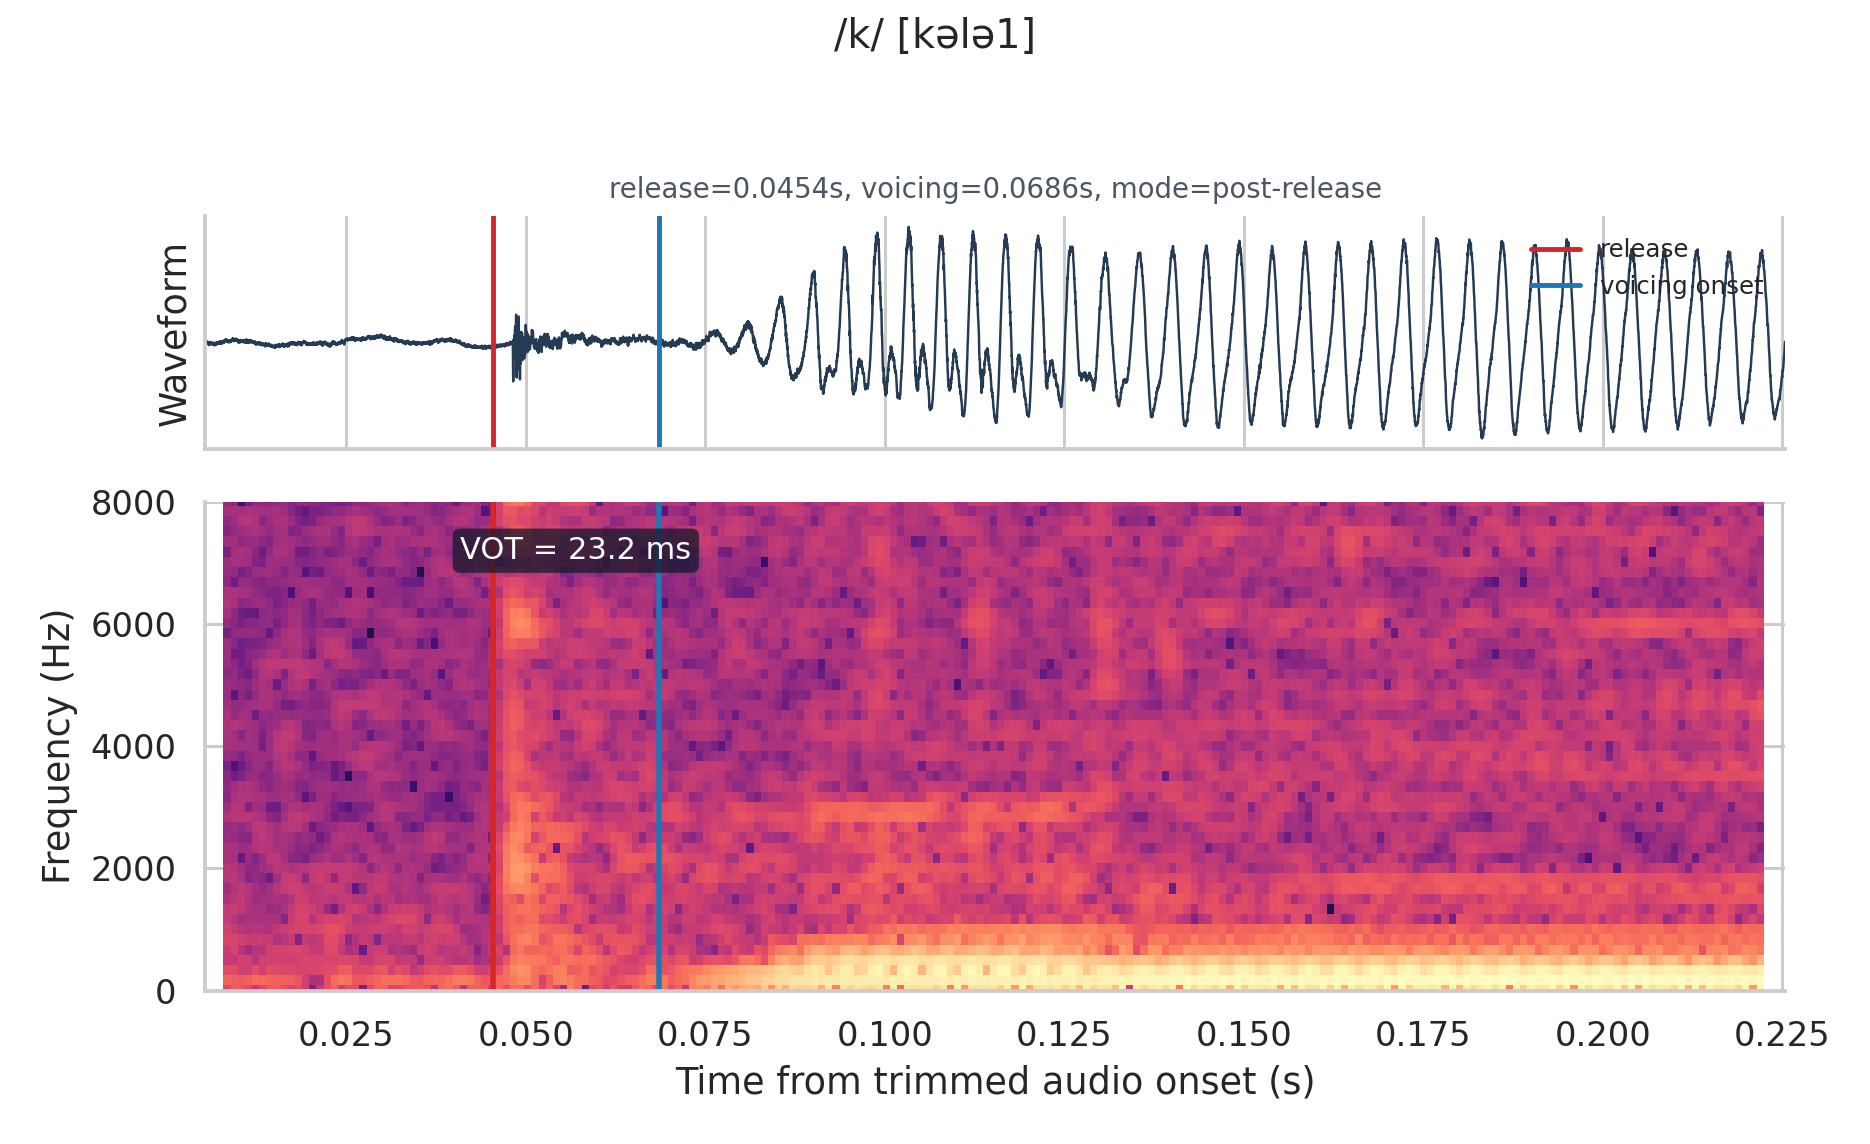
\includegraphics[width=0.8\textwidth]{img/vot_k.png}
\caption{[kələ]“虫子”的发声起始时间}
\label{votk}
\end{figure}

\begin{figure}[H]
\centering
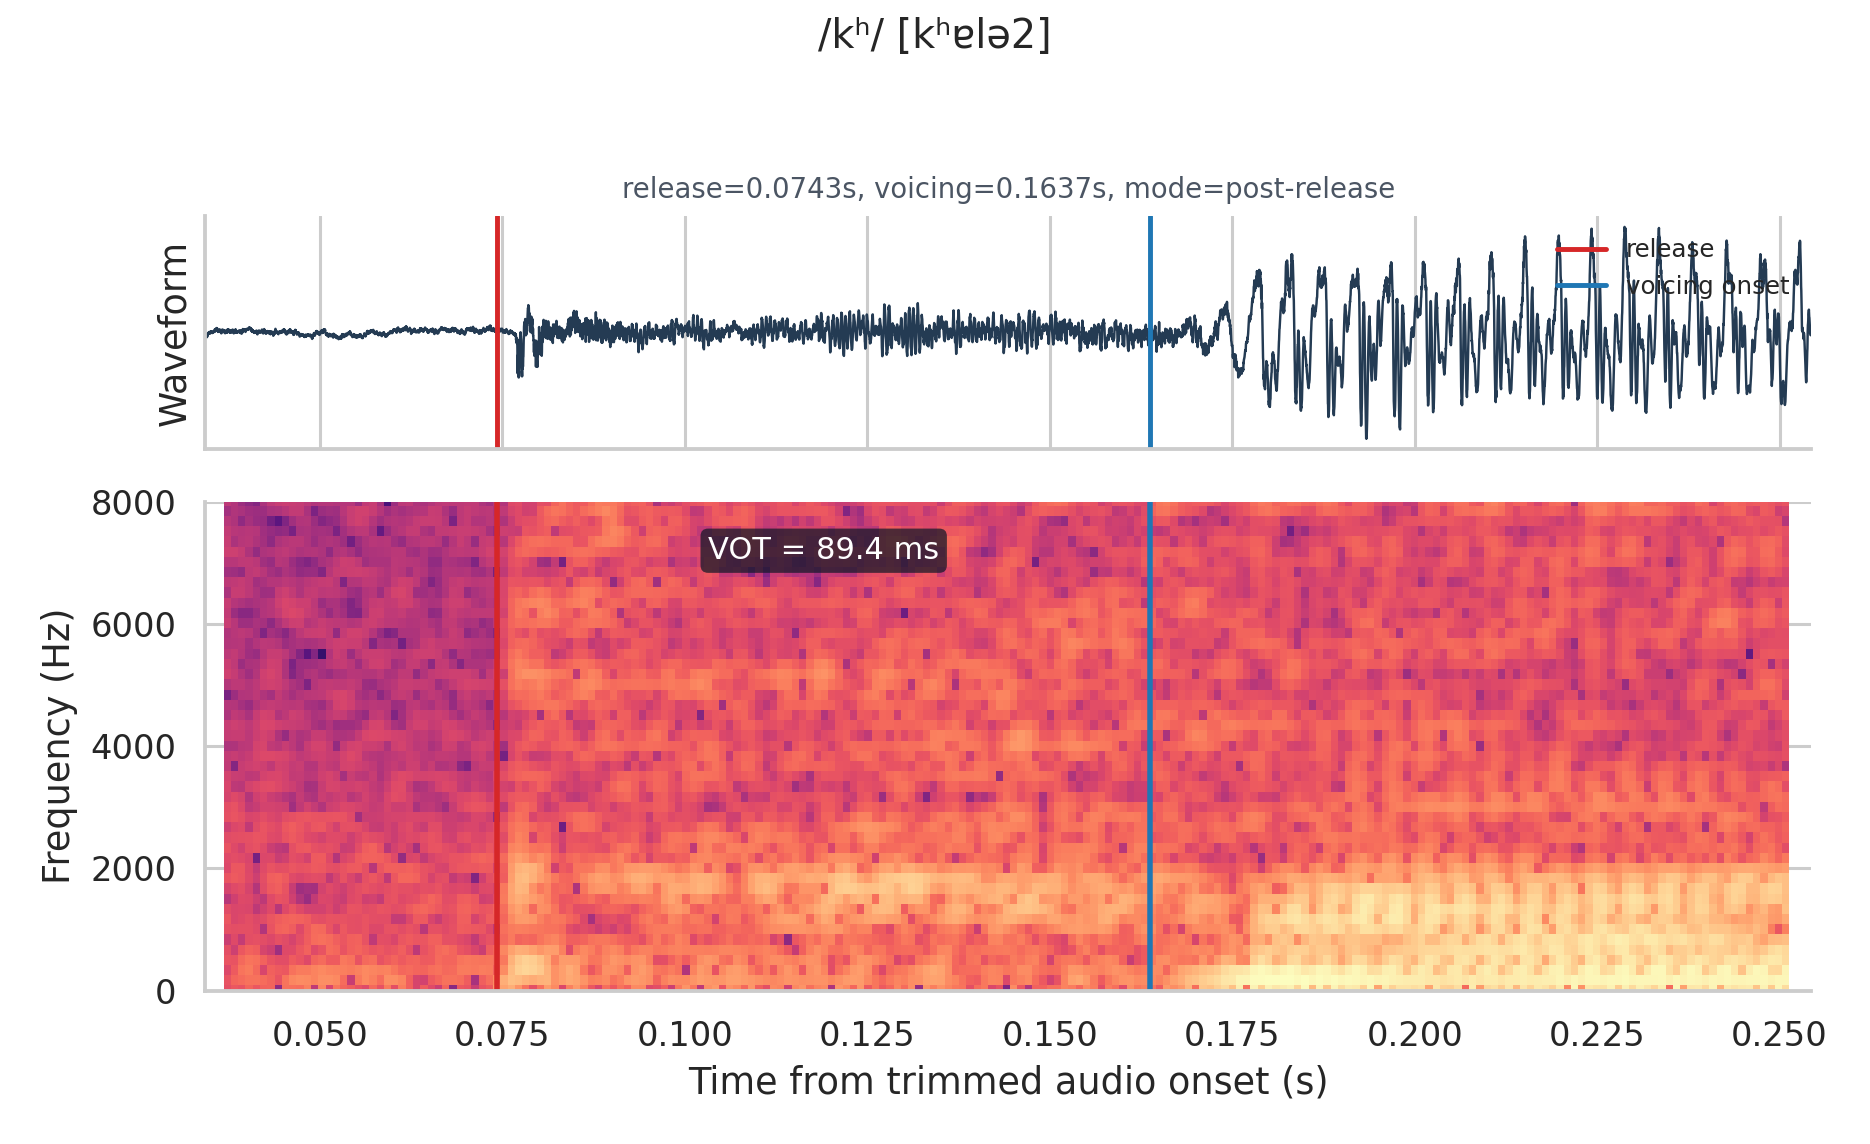
\includegraphics[width=0.8\textwidth]{img/vot_kh.png}
\caption{[kʰɐlə̂]“风”的发声起始时间}
\label{votkh}
\end{figure}

\begin{table}[H]
\vspace{5pt}
\centering
\caption{米亚罗话爆发音的VOT测量}
\label{plosivevot}
\small
\begin{tabular}{ccccc}
\toprule
发音部位 & 类型 & 音位 & 例词 & VOT(ms) \\
\midrule
双唇 & 清不送气 & /p/ & [poji] “老鼠” & +14.1 \\
双唇 & 清送气 & /pʰ/ & [pʰɐtɐk] “面条” & +49.6 \\
双唇 & 浊不送气 & /b/ & [busmuk] “发霉” & -149.8 \\
软腭 & 清不送气 & /k/ & [kələ] “虫子” & +23.2 \\
软腭 & 清送气 & /kʰ/ & [kʰɐlə̂] “风” & +89.4 \\
软腭 & 浊不送气 & /ɡ/ & [ɡən] “很” & -113.0 \\
\bottomrule
\end{tabular}
\end{table}

\subsection{鼻音}

米亚罗话的鼻音有四分对立/m/、/n/、/ɲ/、/ŋ/。表\ref{nasalex}列出了鼻音在元音/o/上的近似最小对。

\begin{table}[H]
\vspace{5pt}
    \centering
    \caption{鼻音的准最小对}
    \label{nasalex}
\begin{tabular}{ccc}
   \toprule
    音位 & 例子 & 释义 \\
   \midrule
   /m/ & [tə-\textbf{mô}] & “母亲”  \\
   /n/ & [\textbf{no}] & “你”  \\
   /ɲ/ & [\textbf{ɲo}] & “你们”  \\
   /ŋ/ & [\textbf{ŋo}] & “我”  \\
   \bottomrule
\end{tabular}
\end{table}

\subsection{擦音}

米亚罗话的擦音存在齿龈、龈后、龈-腭的三分对立。表\ref{fricative}列出了擦音在元音/e/上的近似最小对。

\begin{table}[H]
\vspace{5pt}
    \centering
    \caption{擦音的准最小对}
    \label{fricative}
\begin{tabular}{ccc}
   \toprule
    音位 & 例子 & 释义 \\
   \midrule
   /s/ & [tɐ-\textbf{se}] & “苎麻”  \\
   /ʃ/ & [\textbf{ʃe}] & “生肉”  \\
   /ɕ/ & [tɐ-\textbf{ɕet}] & “梳子”  \\
   /z/ & [kɐ-\textbf{ze}] & “吃”  \\
   /ʒ/ & [kə-\textbf{ʒe}] & “降落” \\
   \bottomrule
\end{tabular}
\end{table}

关于音位/ɕ/和/ʃ/，两者可能处于边缘对立中。/ɕ/几乎只可以与/i/相拼，仅有[tɕukɕu]“鱼”、[tɐ-ɕet]“梳子”、[kɐ-sɐ.ɕet]“梳头”三个反例；而/ʃ/不与/i/相拼。但在元音/u/前有[kʰɐkʃû]“炫耀”，与[tɕukɕu]“鱼”形成对立。但浊音/ʒ/可与/i/相拼（参考/ɕ/对应的同位置浊擦音缺失）。

/s/、/z/也几乎不与/i/相拼，仅有[wu-zər]“旁边”加上位置格后缀-j的形态[wu-zir]一个反例。

另外有软腭擦音/x/，仅出现在汉语借词中，比如形容词/kə-xaw/“好”就是汉语词汇“好”（hǎo）经过重新分析（添加形容词前缀kə-）的结果。


\subsection{塞擦音}

米亚罗话的塞擦音存在清不送气、清送气、浊不送气三分对立，发声部位有齿龈、龈后、龈-腭。表\ref{affricate}列出了塞擦音在元音/a/上的近似最小对。

\begin{table}[H]
\vspace{5pt}
    \centering
    \caption{塞擦音的准最小对}
    \label{affricate}
\begin{tabular}{ccc}
   \toprule
    音位 & 例子 & 释义 \\
   \midrule
   /ts/ & [po-\textbf{tsɐ̂}] & “鸟”  \\
   /tsʰ/ & [\textbf{tsʰɐ̂}] & “盐”  \\
   /dz/ & [\textbf{mdzɐ}ji] & “跳蚤”  \\
   /tʃ/ & [kɐ\textbf{tʃɐ}ʃɿ] & “野草莓”  \\
   /tʃʰ/ & [ʃɐ\textbf{tʃʰɐ̂}] & “地方”  \\
   /dʒ/ & [tə-\textbf{ndʒɐ̂}] & “照片”  \\
   /tɕ/ & [\textbf{tɕɐ}kʰe] & “沟”  \\
   /tɕʰ/ & [\textbf{tɕʰɐ̂}] & “酒”  \\
   /dʑ/ & [\textbf{rdʑɐj}-pû] & “土司/国王”  \\
   \bottomrule
\end{tabular}
\end{table}

在塞擦音中，/dz/、/dʒ/、/dʑ/大部分情况下均带有冠音（n-、r-等），较少单独出现在音节开头。

\subsection{流音及近音}

米亚罗话的流音音位有齿龈颤音/r/、边擦音/ɬ/、边近音/l/。近音音位有双唇音/w/和硬腭音/j/。表\ref{floex}列出了在元音/a/上的准最小对。

\begin{table}[H]
\vspace{5pt}
    \centering
    \caption{流音、近音的准最小对}
    \label{floex}
\begin{tabular}{ccc}
   \toprule
    音位 & 例子 & 释义 \\
   \midrule
   /w/ & [tə-\textbf{wɐ̂}] & “衣服”  \\
   /j/ & [kɐ-nə\textbf{jɐ}] & “抢劫” \\
   /r/ & [kɐ-\textbf{rɐ}lî] & “赔偿”  \\
   /ɬ/ & [\textbf{ɬɐ̂}] & “神”  \\
   /l/ & [\textbf{lɐ}mɐ̂] & “喇嘛”  \\
   \bottomrule
\end{tabular}
\end{table}

音位/ɬ/在米亚罗话中仅见于藏语借词，如/ɬâ/“神”来自藏语\tib{ལྷ།}“神”，/ɬantʃî/“鬼”来自藏语\tib{ལྷ་འདྲེ།}“鬼神”。

\section{词首复辅音}

米亚罗话的声母允许出现最多三个辅音，可以分为冠音C$_{1}$、首音C$_{2}$、介音C$_{3}$。所有的辅音音位都可以作为首音，但冠音和介音只有部分辅音可以担任，如表\ref{premedialex}所示。

\begin{table}[H]
\vspace{5pt}
    \centering
    \caption{冠音、介音允许的辅音}
    \label{premedialex}
\begin{tabular}{cc}
   \toprule
    位置 & 音位 \\
   \midrule
   冠音 &  /k, p, m, n, ŋ, s (z), ʃ (ʒ), r, j, w/ \\
   介音 & /j, w, r, l/ \\
   \bottomrule
\end{tabular}
\end{table}

目前的调查结果，排除只出现在音节边界的复辅音，共得到146种复辅音声母，其中17种由三个辅音组成、129种由两个辅音组成。除了出现在词首的辅音之外，除去前缀（如动词前缀/ka-/、形容词前缀/kə-/等）后剩余音节的起首部分也被纳入统计，因为对于[kɐndwôn]“读”这样的词，唯一可能的音节切分是[kɐ.ndwôn]而非[kɐn.dwôn]。在获得更多证据前，本文暂时排除了[ʃloŋle]“白天”这样的例子，因为不能确定其音节划分是[ʃlo.ŋle]或[ʃloŋ.le]，因此仅出现在此例中的辅音簇/ŋl/没有纳入统计。

为了便于观察组合规律，表\ref{twoconmatrix}列出全部二合复辅音声母，行表示第一辅音，列表示第二辅音，单元格中列出实际出现的二合复辅音，空白单元格表示未见相应组合；表\ref{threeconmatrix}列出全部三合复辅音声母，行表示冠音，列表示介音。

\clearpage

\begin{landscape}
\begin{table}[H]
\vspace{-10pt}
    \centering
    \caption{二合复辅音声母总览}
    \label{twoconmatrix}
\tiny
\setlength{\tabcolsep}{1.5pt}
\renewcommand{\arraystretch}{0.88}
\resizebox{0.93\linewidth}{!}{%
\begin{tabular}{@{}c*{31}{c}@{}}
   \toprule
   & \multicolumn{31}{c}{第二辅音} \\
   \cmidrule(l){2-32}
    第一辅音 & /p/ & /pʰ/ & /b/ & /t/ & /tʰ/ & /d/ & /k/ & /kʰ/ & /ɡ/ & /m/ & /n/ & /ɲ/ & /ŋ/ & /s/ & /z/ & /ʃ/ & /ʒ/ & /ɕ/ & /ts/ & /tsʰ/ & /dz/ & /tʃ/ & /tʃʰ/ & /dʒ/ & /tɕ/ & /tɕʰ/ & /dʑ/ & /r/ & /l/ & /j/ & /w/ \\
   \midrule
   /p/ &  &  &  & pt- &  &  & pk- &  &  &  &  &  &  &  &  & pʃ- &  &  & pts- & ptsʰ- &  & ptʃ- &  &  & ptɕ- &  &  & pr- &  & pj- &  \\
   /pʰ/ &  &  &  &  &  &  &  &  &  &  &  &  &  &  &  &  &  &  &  &  &  &  &  &  &  &  &  & pʰr- &  & pʰj- &  \\
   /m/ & mp- & mpʰ- & mb- & mt- & mtʰ- & md- & mk- &  &  &  & mn- & mɲ- & mŋ- &  &  &  &  &  & mts- & mtsʰ- & mdz- & mtʃ- &  & mdʒ- & mtɕ- &  &  &  &  &  &  \\
   /w/ & wp- &  &  & wt- &  & wd- &  &  & wɡ- & wm- &  &  &  & ws- & wz- & wʃ- & wʒ- & wɕ- &  &  &  & wtʃ- &  &  &  &  &  & wr- & wl- & wj- &  \\
   /t/ &  &  &  &  &  &  &  &  &  &  &  &  &  &  &  &  &  &  &  &  &  &  &  &  &  &  &  &  &  &  & tw- \\
   /tʰ/ &  &  &  &  &  &  &  &  &  &  &  &  &  &  &  &  &  &  &  &  &  &  &  &  &  &  &  &  &  &  & tʰw- \\
   /n/ &  &  &  & nt- & ntʰ- & nd- &  &  &  &  &  &  &  &  &  &  &  &  & nts- & ntsʰ- & ndz- & ntʃ- & ntʃʰ- & ndʒ- & ntɕ- & ntɕʰ- & ndʑ- &  &  &  &  \\
   /s/ & sp- &  &  & st- & stʰ- &  & sk- &  &  & sm- & sn- & sɲ- & sŋ- &  &  &  &  &  &  &  &  &  &  &  & stɕ- &  &  & sr- &  &  & sw- \\
   /z/ &  &  &  &  &  & zd- &  &  & zɡ- &  &  &  &  &  &  &  &  &  &  &  &  &  &  &  &  &  &  &  &  &  &  \\
   /ts/ &  &  &  &  &  &  &  &  &  &  &  &  &  &  &  &  &  &  &  &  &  &  &  &  &  &  &  &  & tsl- &  &  \\
   /r/ & rp- &  & rb- & rt- &  & rd- & rk- & rkʰ- & rɡ- & rm- & rn- & rɲ- & rŋ- &  & rz- &  & rʒ- &  & rts- & rtsʰ- &  & rtʃ- &  &  & rtɕ- &  & rdʑ- &  & rl- & rj- & rw- \\
   /ʃ/ & ʃp- &  &  & ʃt- & ʃtʰ- &  & ʃk- & ʃkʰ- &  & ʃm- & ʃn- &  &  &  &  &  &  &  &  &  &  & ʃtʃ- &  &  & ʃtɕ- &  &  &  & ʃl- &  &  \\
   /ʒ/ &  &  &  &  &  & ʒd- &  &  & ʒɡ- &  &  &  &  &  &  &  &  &  &  &  &  &  &  & ʒdʒ- &  &  &  &  &  &  &  \\
   /tʃ/ &  &  &  &  &  &  &  &  &  &  &  &  &  &  &  &  &  &  &  &  &  &  &  &  &  &  &  &  &  &  & tʃw- \\
   /j/ & jp- & jpʰ- & jb- & jt- &  & jd- & jk- &  &  & jm- & jn- &  & jŋ- &  &  &  &  &  &  &  &  &  &  &  & jtɕ- & jtɕʰ- &  & jr- & jl- &  & jw- \\
   /k/ & kp- &  &  & kt- &  &  &  &  &  &  &  &  &  & ks- &  & kʃ- &  &  & kts- &  &  &  &  &  &  & ktɕʰ- &  & kr- &  &  &  \\
   /kʰ/ &  &  &  &  &  &  &  &  &  &  &  &  &  &  &  &  &  &  &  &  &  &  &  &  &  &  &  &  & kʰl- &  &  \\
   /ŋ/ &  &  &  &  &  &  & ŋk- & ŋkʰ- & ŋɡ- &  &  &  &  &  &  &  &  &  &  &  &  &  &  &  &  &  &  &  &  &  &  \\
   \bottomrule
\end{tabular}%
}
\end{table}
\end{landscape}

\clearpage

\begin{table}[H]
\vspace{5pt}
    \centering
    \caption{三合复辅音声母总览}
    \label{threeconmatrix}
\small
\setlength{\tabcolsep}{6pt}
\renewcommand{\arraystretch}{1.15}
\begin{tabular}{c|cccc}
   \toprule
    冠音 & 介音/j/ & 介音/w/ & 介音/r/ & 介音/l/ \\
   \midrule
   /m/ & \makecell[l]{mpʰj-} &  & \makecell[l]{mbr-\\ mkr-} &  \\
   /n/ & \makecell[l]{npj-} & \makecell[l]{ntw-} &  &  \\
   /s/ & \makecell[l]{spj-} &  & \makecell[l]{skr-} & \makecell[l]{spl-} \\
   /z/ &  &  & \makecell[l]{zbr-\\ zɡr-} &  \\
   /ʃ/ &  &  & \makecell[l]{ʃkr-} & \makecell[l]{ʃkl-} \\
   /ʒ/ &  &  & \makecell[l]{ʒɡr-} &  \\
   /j/ &  &  & \makecell[l]{jkr-} &  \\
   /k/ & \makecell[l]{kpj-} &  & \makecell[l]{kpr-} &  \\
   /ŋ/ &  &  & \makecell[l]{ŋkr-} &  \\
   \bottomrule
\end{tabular}
\end{table}

\subsection{冠音}

米亚罗话的冠音位置能够出现10个辅音音位，分别是/k, p, m, n, ŋ, s (z), ʃ (ʒ), r, j, w/。冠音位置的辅音清浊对立中和。

\subsubsection{/k/作为冠音}

/k/可以作为8个复辅音的冠音，如表\ref{kpre}所示。

\begin{table}[H]
\vspace{5pt}
    \centering
    \caption{/k/作为冠音的复辅音}
    \label{kpre}
\begin{tabular}{c|cccc}
     \toprule
复辅音   & 示例              & 释义   & 无冠音示例          & 释义        \\
     \midrule
	kpr-  & {[}tə-kprî{]}  & 口信   & {[}kɐ-pri{]}   & 撕         \\
kpj-  & {[}tɐ-kpje{]}   & 辫子   & {[}kɐ-pje{]}   & 捉/拿/钓鱼    \\
kp-   & {[}tə-kpe{]}    & 庄稼   & {[}pe{]}       & 鸡         \\
ks-   & {[}kɐ-ksə̂r{]}  & 炒（菜） & {[}kə-sə̂k{]}  & 沙哑/紧      \\
kʃ-   & {[}kʃɿ{]}       & 米    & {[}tə-ʃɿ{]}    & 水果        \\
kt-   & {[}kə-ktî{]}   & 大的   & {[}ŋɐ-tî{]}   & （我的）大叔/大舅 \\
ktɕʰ- & {[}kə-ktɕʰî{]} & 远的   & {[}kɐ-tɕʰî{]} & 去         \\
kts-  & {[}tə-ktse{]}   & 鞋子   & {[}tə-tse{]}   & 男人/儿子    \\ 
   \bottomrule
\end{tabular}
\end{table}

\subsubsection{/p/作为冠音}

/p/可以作为7个复辅音的冠音，如表\ref{ppre}所示。

\begin{table}[H]
\vspace{5pt}
    \centering
    \caption{/p/作为冠音的复辅音}
    \label{ppre}
\begin{tabular}{c|cccc}
     \toprule
复辅音   & 示例              & 释义   & 无冠音示例          & 释义        \\
     \midrule
	pk-  & {[}kə-pkɐ̂{]}      & 饱的        & {[}kɐ-{]}      & 动词词典形前缀 \\
pʃ-  & {[}kɐ-pʃɐ̂m{]}     & 晒谷子/散开/撒落 & {[}ʃɐmtə{]}    & 枪       \\
pt-  & {[}kɐ-nə.ptekpe{]} & 崇拜        & {[}te-{]}      & 一（数量前缀） \\
ptɕ- & {[}wu-ptɕis{]}     & 方向        & {[}kɐ-tɕi{]}   & 泼       \\
pts- & {[}kɐ-ptsə̂m{]}    & 闭嘴        & {[}kə-tsə̂r{]} & 咸的      \\
ptʃ  & {[}kɐ-ptʃɿ̂{]}     & 熬油/煎/融化   & {[}tə-tʃɿ{]}   & 水       \\
ptsʰ & {[}mɐ-kə-ptsʰi{]}  & 不得不       & {[}tsʰɐ̂{]}    & 盐      \\ 
   \bottomrule
\end{tabular}
\end{table}

\subsubsection{/m/作为冠音}

/m/可以作为19个复辅音的冠音，如表\ref{mpre}所示。

\begin{table}[H]
\vspace{5pt}
    \centering
    \caption{/m/作为冠音的复辅音}
    \label{mpre}
\begin{tabular}{c|cccc}
     \toprule
复辅音   & 示例              & 释义   & 无冠音示例          & 释义        \\
     \midrule
	mbr-  & {[}mbro{]}         & 马         & {[}brɐrî{]}   & 地震      \\
mb-   & {[}mbole{]}        & 公牛        & {[}boŋti{]}    & 裹腿      \\
md-   & {[}kɐ-mdə̂{]}      & 到         & {[}tɐ-dok{]}   & 毒药      \\
mdz-  & {[}tə-mdzu{]}      & 刺         &                &         \\
mdʒ-  & {[}tə-mdʒe{]}      & 下巴        & {[}tə-dʒɿ̂{]}  & 皮肤      \\
mkr-  & {[}tə-mkrə̂m{]}    & 喉结        & {[}tə-krə{]}   & 手肘      \\
mk-   & {[}tə-mkɤ{]}       & 脖子        & {[}kɐ-kɤ̂{]}   & 买       \\
mn-   & {[}kə-mni{]}       & 少的        & {[}nizən{]}    & 日食      \\
mɲ-   & {[}kɐ-mɲô{]}      & 准备        & {[}ɲo{]}       & 你们      \\
mŋ-   & {[}kə-mŋân{]}     & 低的/便宜的    & {[}tɐ-ŋɐj{]}   & 太阳      \\
mp-   & {[}wu-mpu{]}       & 外面        & {[}tə-pû{]}   & 肠子      \\
mpʰj- & {[}kə-mpʰjêr{]}   & 漂亮的       & {[}te-pʰjɐr{]} & 一张/一片   \\
mpʰ-  & {[}kɐ-mpʰɐr{]}     & 卖         & {[}tə-pʰɐje{]} & 丈夫      \\
mt-   & {[}tə-mto{]}       & 额头        & {[}to{]}       & 上（n.）   \\
mtɕ-  & {[}kɐ-mtɕî{]}     & 要         & {[}tə-tɕi{]}   & 弟弟/妹妹   \\
mtʰ-  & {[}tə-mtʰek{]}     & 腰         & {[}tʰe{]}      & 什么      \\
mts-  & {[}kɐ-mtsɿ{]}      & 钉/钉子      & {[}kə-tsɿ{]}   & 猴子      \\
mtsʰ- & {[}kə-wɐ.mtsʰɐr{]} & 奇怪的/莫名其妙的 & {[}kə-tsʰɐr{]} & 闪光的/清楚的 \\
mtʃ-  & {[}tə-mtʃək{]}     & 火         & {[}tɐ-tʃək{]}  & 芽      \\ 
   \bottomrule
\end{tabular}
\end{table}

在一些嘉绒语组语言，例如草登嘉绒语\cite{sun1994caodeng}、茶堡嘉绒语\cite{jacques2021grammar}、四土嘉绒语白湾话\cite{zhang2016phonologie}中，在同部位浊爆发音、浊塞擦音之前的鼻冠音会被分析为带鼻冠色彩的单辅音。这样分析的理由是鼻冠爆发音、塞擦音可以与其他冠音结合，形成形如znd-这样的复辅音。然而在米亚罗话中，这样的现象没有被观察到，因此本文暂将所有鼻冠音分析为二合复辅音。

\subsubsection{/n/作为冠音}

/n/可以作为15个复辅音的冠音，如表\ref{npre}所示。

\begin{table}[H]
\vspace{5pt}
    \centering
    \caption{/n/作为冠音的复辅音}
    \label{npre}
\begin{tabular}{c|cccc}
     \toprule
复辅音   & 示例              & 释义   & 无冠音示例          & 释义        \\
     \midrule
	nd-   & {[}ka-ndu{]}       & 得到    & {[}tɐ-dok{]}    & 毒药      \\
ndz-  & {[}ta-ndzûj{]}    & 动物的牙  &                 &         \\
ndʒ-  & {[}tə-ndʒɐ̂{]}     & 照片    & {[}tə-dʒɿ̂{]}   & 皮肤      \\
ndʑ-  & {[}ndʑolî{]}         & 笛子    &     {[}dʑu{]}         & 竹子  \\
npj-  & {[}kə-npjôk{]}    & 软的    & {[}tɐ-pju{]}    & 毯子      \\
ntw-  & {[}tə-ntwe{]}      & 镰刀    & {[}kɐ-twe{]}    & 割       \\
nt-   & {[}ta-nter{]}      & 垃圾/灰尘 & {[}tɐ-ter{]}    & 棍子      \\
ntɕ-  & {[}ta-ntɕep{]}     & 山阴    & {[}kə-tɕep{]}   & 苦的      \\
ntɕʰ- & {[}ta-ntɕʰî{]}    & 柱子/楔子 & {[}kɐ-tɕʰî{]}  & 去       \\
ntʰ-  & {[}kə-ntʰɐ̂m{]}    & 平的    & {[}tʰɐm{]}      & 虽然/如果   \\
nts-  & {[}te-ntsok{]}     & 有点    & {[}kʰotsôk{]}  & 佛堂旁的房间  \\
ntsʰ- & {[}kɐ-nə-ntsʰok{]} & 舔     & {[}kɐ-tsʰôk{]} & 犁（地）/贴近 \\
ntʃ-  & {[}ka-ntʃɿ̂{]}     & 搬     & {[}tə-tʃɿ{]}    & 水       \\
ntʃʰ- & {[}ka-ntʃʰe{]}     & 杀/宰   & {[}kə-tʃʰɿ̂{]}  & 甜的     \\ 
   \bottomrule
\end{tabular}
\end{table}

\subsubsection{/ŋ/作为冠音}

/ŋ/可以作为4个复辅音的冠音，如表\ref{ngpre}所示。

\begin{table}[H]
\vspace{5pt}
    \centering
    \caption{/ŋ/作为冠音的复辅音}
    \label{ngpre}
\begin{tabular}{c|cccc}
     \toprule
复辅音   & 示例              & 释义   & 无冠音示例          & 释义        \\
     \midrule
	ŋɡ-  & {[}tɑ-ŋɡɤ̂{]}      & 背部 & {[}wu-ɡɤ{]}  & 里面 \\
ŋkr- & {[}kɐ-nə-ŋkrôs{]} & 分手 & {[}kɐ-kro{]} & 分  \\
ŋk-  & {[}kə-ŋkôr{]}     & 脏的 & {[}kɐ-kor{]} & 帮助 \\
ŋkʰ- & {[}kə-ŋkʰân{]}    & 多的 & {[}kʰanpu{]} & 堪布\\ 
   \bottomrule
\end{tabular}
\end{table}

\subsubsection{/s (z)/作为冠音}

/s/可以作为15个复辅音的冠音。在冠音位置上，/s/和/z/对立中和，在首音辅音是浊音时表层为/z/。如表\ref{spre}所示。

\begin{table}[H]
\vspace{5pt}
    \centering
    \caption{/s (z)/作为冠音的复辅音}
    \label{spre}
\begin{tabular}{c|cccc}
     \toprule
复辅音   & 示例              & 释义   & 无冠音示例          & 释义        \\
     \midrule
	sp-  & {[}spos{]}        & 熏香       & {[}tɐ-pôs{]}   & 奴隶    \\
st-  & {[}ka-stə̂{]}     & 敲击/打铁    & {[}kɐ-tə̂{]}    & 开门/打开 \\
stɕ- & {[}kə-stɕî{]}    & 生的       & {[}tɐ-tɕî{]}   & 锁     \\
stʰ- & {[}kɐ-stʰêt{]}   & 取（名）/取得  & {[}tʰe{]}       & 什么    \\
sk-  & {[}tə-ske{]}      & 声音       & {[}tɐ-ke{]}     & 蹄子    \\
sm-  & {[}kə-smî{]}     & 熟的       & {[}tɐ-mî{]}    & 脚     \\
sn-  & {[}kə-snɐ̂{]}     & 好的       & {[}kɐ-nɐ.kʰu{]} & 喊     \\
sɲ-  & {[}tɐ-sɲɐ.tsɐ̂{]} & 一种绳子上的装饰 & {[}tɐ-ɲɐt{]}    & 塌方    \\
sŋ-  & {[}sŋɐ̂r{]}       & 霜        & {[}tɐ-ŋɐj{]}    & 太阳    \\
zd-  & {[}zdem{]}        & 云        & {[}tɐ-dok{]}    & 毒药    \\
zɡ-  & {[}zɡɐ̂r{]}       & 帐篷       & {[}tɐ-ɡɐm{]}    & 蛋    \\ 
skr- & {[}tə-skrə{]}   & 身体     & {[}tə-krə{]}    & 手肘    \\
spl- & {[}sple{]}      & 佛堂前的阳台 & {[}kɐ-ʃɐ.plo{]} & 耽误    \\
zbr- & {[}tɐ-zbro{]}   & 踢      & {[}brɐrî{]}    & 地震    \\
zɡr- & {[}zɡrôks{]}   & 手镯     &                 &       \\
   \bottomrule
\end{tabular}
\end{table}

\subsubsection{/ʃ (ʒ)/作为冠音}

/ʃ/可以作为15个复辅音的冠音。在冠音位置上，/ʃ/和/ʒ/对立中和，在首音辅音是浊音时表层为/ʒ/。如表\ref{sspre}所示。

\begin{table}[H]
\vspace{5pt}
    \centering
    \caption{/ʃ (ʒ)/作为冠音的复辅音}
    \label{sspre}
\begin{tabular}{c|cccc}
     \toprule
复辅音   & 示例              & 释义   & 无冠音示例          & 释义        \\
     \midrule
	ʃk-  & {[}kɐ-ʃkət{]}   & 吃完   & {[}kɐ-kɤ̂{]}  & 买     \\
ʃkʰ- & {[}tə-ʃkʰor{]}  & 疮    & {[}kʰô{]}    & 房间    \\
ʃm-  & {[}tə-ʃmî{]}   & 舌头   & {[}tɐ-mî{]}  & 脚     \\
ʃn-  & {[}te-ʃnə̂{]}   & 一天   & {[}tə-nə{]}   & 乳房    \\
ʃp-  & {[}kə-ʃpə{]}    & 畜牲   & {[}pə{]}      & 现在    \\
ʃt-  & {[}kɐ-ʃti{]}    & 塞/捂嘴 & {[}ŋɐ-tî{]}  & 大叔/大舅 \\
ʃtɕ- & {[}ʃtɕi{]}      & 10   & {[}tə-tɕi{]}  & 弟弟/妹妹 \\
ʃtʰ- & {[}tə-ʃtʰêk{]} & 大腰带  & {[}tʰe{]}     & 什么    \\
ʃtʃ- & {[}tɐ-ʃtʃɿ{]}   & 尿    & {[}tə-tʃɿ{]}  & 水     \\
ʒd-  & {[}kə-ʒdɐ̂r{]}  & 紧张的  & {[}tɐ-dok{]}  & 毒药    \\
ʒdʒ- & {[}kɐ-ʒdʒɿ̂{]}  & 剥皮   & {[}tə-dʒɿ̂{]} & 皮肤    \\
ʒɡ-  & {[}kɐ-ʒɡə{]}    & 砍    & {[}tɐ-ɡɐm{]}  & 蛋    \\ 
ʃkl- & {[}kɐwlɐ.ʃklɐ̂k{]} & 左撇子  &               &       \\
ʃkr- & {[}wu-ʃkre{]}      & 附近   & {[}tə-krə{]}  & 手肘    \\
ʒɡr- & {[}ʒɡrək{]}        & 一定   &               &       \\
   \bottomrule
\end{tabular}
\end{table}

\subsubsection{/r/作为冠音}

/r/可以作为18个复辅音的冠音，如表\ref{rpre}所示。

\begin{table}[H]
\vspace{5pt}
    \centering
    \caption{/r/作为冠音的复辅音}
    \label{rpre}
\begin{tabular}{c|cccc}
     \toprule
复辅音   & 示例              & 释义   & 无冠音示例          & 释义        \\
     \midrule
	rm-   & {[}tə-rmî{]}   & 名字     & {[}tɐ-mî{]}  & 脚          \\
rn-   & {[}kə-rnɐk{]}   & 深的     & {[}te-nɐ̂k{]} & 早上         \\
rɲ-   & {[}tɐ-rɲi{]}    & 毛      & {[}əɲî{]}    & 我们（排除式）    \\
rŋ-   & {[}kɐ-rŋɤ̂{]}   & 蹲      & {[}ŋə-{]}     & 第一人称单数领属前缀 \\
rp-   & {[}tə-rpə{]}    & 种子     & {[}pə{]}      & 现在         \\
rt-   & {[}tɐ-rtə{]}    & 帽子     & {[}kɐ-tə̂{]}  & 开门/打开      \\
rk-   & {[}tɐ-rkɤ{]}    & 拳头     & {[}kɐ-kɤ̂{]}  & 买          \\
rkʰ-  & {[}tɐ-rkʰôm{]} & 翅膀     & {[}kʰô{]}    & 房间         \\
rtɕ-  & {[}kɐ-rtɕik{]}  & 跑/逃走   & {[}tə-tɕi{]}  & 弟弟/妹妹      \\
rdʑ-  & {[}kə-rdʑôm{]} & 宽的     &   {[}dʑu{]}         & 竹子 \\
rd-   & {[}kə-rdə̂k{]}  & 累的     & {[}tɐ-dok{]}  & 毒药         \\
rb-   & {[}tə-rbo{]}    & 锣/鼓/钟  & {[}boŋti{]}   & 裹腿         \\
rɡ-   & {[}kə-rgɤ{]}    & 牦牛     & {[}tɐ-ɡɐm{]}  & 蛋          \\
rts-  & {[}tə-rtsɐ̂{]}  & 铁锈/脉搏  & {[}potsɐ̂{]}  & 鸟          \\
rtsʰ- & {[}tə-rtsʰes{]} & 肺/咳嗽/痰 & {[}kə-tsʰu{]} & 胖的         \\
rtʃ-  & {[}tɐ-rtʃok{]}  & 经幡     & {[}kə-tʃok{]} & 6          \\
rʒ-   & {[}tɐ-rʒep{]}   & 妻子     & {[}kə-ʒe{]}   & 掉/降落       \\
rz-   & {[}kɐ-rzək{]}   & 剪/绞掉   & {[}wu-zər{]}  & 旁边        \\
   \bottomrule
\end{tabular}
\end{table}

\subsubsection{/j/作为冠音}

/j/可以作为13个复辅音的冠音，如表\ref{jpre}所示。

\begin{table}[H]
\vspace{5pt}
    \centering
    \caption{/j/作为冠音的复辅音}
    \label{jpre}
\begin{tabular}{c|cccc}
     \toprule
复辅音   & 示例              & 释义   & 无冠音示例          & 释义        \\
     \midrule
	jm-   & {[}tɐ-jmə{]}      & 尾巴      & {[}tə-mə{]}    & 女人/女儿   \\
jn-   & {[}tə-jnô{]}     & 菜肴/蔬菜   & {[}no{]}       & 你       \\
jŋ-   & {[}kə-jŋu{]}      & 发誓      & {[}nəŋe{]}     & 牛       \\
jp-   & {[}tɐ-jpet{]}     & 雪       & {[}tɐ-pet{]}   & 面粉      \\
jpʰ-  & {[}kə-ŋa.jpʰit{]} & 遗失（不及物） & {[}kɐ-pʰît{]} & 扔/掷/吐/丢 \\
jk-   & {[}jkɐ̂r{]}       & 铜/绿松石   & {[}kɐ-kɤ̂{]}   & 买       \\
jkr-  & {[}tə-jkrôm{]}   & 院子      & {[}kɐ-kro{]}   & 分       \\
jtɕ-  & {[}ʃko.jtɕî{]}   & 水芹菜     & {[}tə-tɕi{]}   & 弟弟/妹妹   \\
jtɕʰ- & {[}ʃko.jtɕʰê{]}  & 飘带葱     & {[}kɐ-tɕʰe{]}  & 右面/右手   \\
jd-   & {[}kɐ-jdɐ̂{]}     & 解开      & {[}tɐ-dok{]}   & 毒药      \\
jb-   & {[}kə-jbɐm{]}     & 粗的      & {[}boŋti{]}    & 裹腿      \\
jt-   & {[}tɐ-jtu{]}      & 萝卜      & {[}kɐ-tup{]}   & 打      \\
   \bottomrule
\end{tabular}
\end{table}

\subsubsection{/w/作为冠音}

/w/可以作为11个复辅音的冠音，如表\ref{wpre}所示。

\begin{table}[H]
\vspace{5pt}
    \centering
    \caption{/w/作为冠音的复辅音}
    \label{wpre}
\begin{tabular}{c|cccc}
     \toprule
复辅音   & 示例              & 释义   & 无冠音示例          & 释义        \\
     \midrule
	wɕ-  & {[}tə-wɕi{]}    & 肝   & {[}ɕi{]}         & 柴火   \\
wɡ-  & {[}kɐ-wɡû{]}   & 进来  & {[}kɐ-ɡû{]}     & 钻    \\
wm-  & {[}tɐ-wmô{]}   & 祖母  & {[}tə-mô{]}     & 母亲   \\
wp-  & {[}tɐ-wpɐ̂{]}   & 祖父  & {[}tɐ-pɐ̂{]}     & 父亲   \\
ws-  & {[}kə-wsu{]}    & 相似的 & {[}kə-rəsusû{]} & 活的   \\
wʃ-  & {[}kɐ-rɐ.wʃɿ{]} & 撕开  & {[}tɐ-ʃɿ{]}      & 血    \\
wt-  & {[}kə-wtîn{]}  & 好的  & {[}tik{]}        & 1    \\
wtʃ- & {[}kɐ-wtʃî{]}  & 走   & {[}tʃi{]}        & 黄鼠狼  \\
wz-  & {[}tə-wzûs{]}  & 木匠  & {[}kə-zûr{]}    & 痛的   \\
wʒ-  & {[}kɐ-wʒɐ̂r{]}  & 剃头  & {[}ʒɐlɐ̂{]}      & 糊（墙）\\
wd- & {[}kə-wdə̂{]}  & 4  & {[}tɐ-dok{]}   & 毒药      \\
   \bottomrule
\end{tabular}
\end{table}

\subsection{介音}

米亚罗话复辅音声母可以独立出明确的介音。考察三个辅音组成的复辅音声母（如表\ref{comconex}）可以发现，C$_{3}$位置仅可能出现四种辅音：/w, j, r, l/。这四个辅音均是流音或近音，音质上经常作为过渡音出现，因此归纳出介音是合理的。

\begin{table}[H]
\vspace{5pt}
    \centering
    \caption{三合复辅音示例}
    \label{comconex}
\begin{tabular}{ccc|ccc}
     \toprule
	/mbr/ & [kɐ-mbrî] & 玩耍 & /ʃkl/ & [kɐwlɐ ʃklɐk] & 左撇子 \\
	/ntw/ & [tə-ntwe] & 镰刀 & /skr/ & [kə-skrîn] & 长的 \\
	/kpj/ & [tɐ-kpje] & 辫子 & /spl/ & [sple] & 佛堂前的阳台 \\
	/zbr/ & [tɐ-zbro] & 踢 & /mkr/ & [kə-ŋa-mkrɐk] & 横着的 \\
	/zɡr/ & [zɡroks] & 手镯 & /npj/ & [kə-npjôk] & 软的 \\
	/ʃkr/ & [ʃkre] & 筛子 & /mpʰj/ & [kə-mpʰjer] & 美丽的 \\ 
	/ʒɡr/ & [ʒɡrək] & 一定 & /kpr/ & [tə-kprî] & 口信 \\ 
	/ŋkr/ & [kɐ-nə-ŋkrôs] & 分手 & /jkr-/ & [tə-jkrôm] & 院子 \\ 
   \bottomrule
\end{tabular}
\end{table}

\subsubsection{/j/作为介音}

/j/可以作为5个复辅音的介音，如表\ref{jmid}所示。

\begin{table}[H]
\vspace{5pt}
    \centering
    \caption{/j/作为介音的复辅音}
    \label{jmid}
\begin{tabular}{c|cccc}
     \toprule
复辅音   & 示例              & 释义   & 无介音示例          & 释义        \\
     \midrule
	kpj-  & {[}tɐ-kpje{]}   & 辫子  & {[}tə-kpe{]}   & 庄稼    \\
mpʰj- & {[}kә-mpʰjer{]} & 美丽的 & {[}tɐ-mpʰej{]} & 补丁    \\
npj-  & {[}kə-npjôk{]} & 软的  &                &       \\
pj-   & {[}tɐ-pju{]}    & 毯子  & {[}tə-pû{]}   & 肠子    \\
pʰj-  & {[}pʰjɐks{]}    & 磕头  & {[}kɐ-pʰɐ̂k{]} & 砍柴/拆开 \\
   \bottomrule
\end{tabular}
\end{table}

\subsubsection{/w/作为介音}

/w/可以作为4个复辅音的介音，如表\ref{wmid}所示。

\begin{table}[H]
\vspace{5pt}
    \centering
    \caption{/w/作为介音的复辅音}
    \label{wmid}
\begin{tabular}{c|cccc}
     \toprule
复辅音   & 示例              & 释义   & 无介音示例          & 释义        \\
     \midrule
	ntw- & {[}tə-ntwe{]}   & 镰刀 & {[}ta-nter{]}  & 垃圾/灰尘 \\
tw-  & {[}kɐ-twe{]}    & 割  & {[}tej{]}      & 麦子    \\
tʰw- & {[}kɐ-tʰwɐt{]}  & 挑刺 & {[}tə-tʰɐ̂{]}  & 书     \\
tʃw- & {[}kɐ-tʃwɐk{]}  & 撬  & {[}kɐ-tʃɐk{]}  & 推/压/按 \\
   \bottomrule
\end{tabular}
\end{table}

\subsubsection{/r/作为介音}

/r/可以作为13个复辅音的介音，如表\ref{rmid}所示。

\begin{table}[H]
\vspace{5pt}
    \centering
    \caption{/r/作为介音的复辅音}
    \label{rmid}
\begin{tabular}{c|cccc}
     \toprule
复辅音   & 示例              & 释义   & 无介音示例          & 释义        \\
     \midrule
	jkr- & {[}tə-jkrôm{]}    & 院子  & {[}jkɐ̂r{]}    & 铜/绿松石 \\
kpr- & {[}tə-kprî{]}     & 口信  & {[}tə-kpə̂n{]} & 和尚    \\
mbr- & {[}mbro{]}         & 马   & {[}mbô{]}     & 舀水瓢   \\
mkr- & {[}kə-ŋa-mkrɐk{]}  & 横着的 & {[}tɐ-mkɐ̂m{]} & 枕头    \\
ŋkr- & {[}kɐ-nə-ŋkrôs{]} & 分手  & {[}kə-ŋkôr{]} & 脏的    \\
skr- & {[}kə-skrîn{]}    & 长的  & {[}skɤ̂{]}     & 佛     \\
ʃkr- & {[}ʃkre{]}         & 筛子  & {[}kɐ-ʃkət{]}  & 吃完    \\
zbr- & {[}tɐ-zbro{]}      & 踢   & {[}zbɐjkʰok{]} & 乌龟    \\
zɡr- & {[}zɡroks{]}       & 手镯  & {[}zɡɐ̂r{]}    & 帐篷    \\
ʒɡr- & {[}ʒɡrək{]}        & 一定  & {[}kɐ-ʒɡɤ{]}   & 砍     \\
kr-  & {[}tə-krə{]}       & 手肘  & {[}kɐ-kɤ̂{]}   & 买     \\
pr-  & {[}tɐ-prə{]}       & 晚饭  & {[}pə{]}       & 现在    \\
pʰr- & {[}kɐ-pʰrôŋ{]}    & 呛   & {[}kɐ-pʰô{]}  & 躲    \\
   \bottomrule
\end{tabular}
\end{table}

\subsubsection{/l/作为介音}

/l/可以作为4个复辅音的介音，如表\ref{lmid}所示。

\begin{table}[H]
\vspace{5pt}
    \centering
    \caption{/l/作为介音的复辅音}
    \label{lmid}
\begin{tabular}{c|cccc}
     \toprule
复辅音   & 示例              & 释义   & 无介音示例          & 释义        \\
     \midrule
	spl- & {[}sple{]}        & 佛堂前的阳台 & {[}te-spû{]}  & 一群    \\
ʃkl- & {[}kɐwlɐ ʃklɐk{]} & 左撇子    & {[}kɐ-ʃkət{]}  & 吃完    \\
kʰl- & {[}tɐ-kʰlê{]}    & 袖子     & {[}tʃʰɿ.kʰe{]} & 河     \\
tsl- & {[}tsle{]}        & 月份     & {[}tə-tse{]}   & 男人/儿子\\
   \bottomrule
\end{tabular}
\end{table}

\subsection{结构歧义的复辅音}

对于由二合复辅音声母，最后一个辅音是/w, j, r, l/之一的可能会出现结构歧义，因为它们结构上既可以是首音也可以是介音。表\ref{ambicom}列出了米亚罗话中所有可能的最后一个辅音是/w, j, r, l/的二合复辅音，并将其分为有证据认为是首音-介音结构、和不能确定是首音-介音或冠音-首音结构的两类。

\begin{table}[H]
\centering
\caption{米亚罗话以 /w, j, r, l/ 结束的二合复辅音}
\label{ambicom}
\begin{tabular}{c|cccc}
\toprule
 & /w/ & /j/ & /r/ & /l/ \\
\midrule
首音-介音
 & \makecell[l]{tw-\\ tʰw-\\ tʃw-}
 & \makecell[l]{pj-\\ pʰj-}
 & \makecell[l]{kr-\\ pr-\\ pʰr-}
 & \makecell[l]{kʰl-\\ tsl-} \\
\midrule
结构歧义
 & \makecell[l]{jw-\\ rw-\\ sw-}
 & \makecell[l]{rj-\\ wj-}
 & \makecell[l]{jr-\\ sr-\\ wr-}
 & \makecell[l]{jl-\\ rl-\\ wl-\\ ʃl-} \\
\bottomrule
\end{tabular}
\end{table}

其中，虽然/pj/、/kr/、/pr/三个复辅音也可以分析成/k/、/p/作为冠音而/j/、/r/作为首音，但鉴于存在/npj/、/skr/、/kpr/这样的三合复辅音的例子，在发现更多证据之前，在分布上将爆发音-流音/近音的组合统一归为首音-介音更为合理。

本文暂不将存在结构歧义的复辅音纳入冠音或介音的分析中。这些复辅音的示例如表\ref{ambiex}。

\begin{table}[H]
\vspace{5pt}
    \centering
    \caption{结构歧义复辅音示例}
    \label{ambiex}
\begin{tabular}{ccc|ccc}
     \toprule
jw- & {[}tɐ-jwɐk{]} & 隔壁     & sr- & {[}tə-srɐm{]}   & 根     \\
rw- & {[}tɐ-rwu{]}  & 蓑衣     & wr- & {[}tə-wri{]}    & 绳子    \\
sw- & {[}tə-swe{]}  & 牙齿     & jl- & {[}tɐ-jlêps{]} & 尘土/蒸汽 \\
rj- & {[}tə-rju{]}  & 语言     & wl- & {[}kə-wlû{]}   & 浑浊的   \\
wj- & {[}tɐ-wje{]}  & 瘸子     & rl- & {[}kə-rlɐk{]}   & 乌鸦    \\
jr- & {[}kɐ-jrû{]} & 寻找（近处） & ʃl- & {[}tə-ʃlɐ̂{]}   & 玩笑   \\ 
   \bottomrule
\end{tabular}
\end{table}

\section{零声母音节} \label{zero}

米亚罗话一些词汇可以以零声母音节开头。零声母的音节仅限/ə/和/a/。例如[əʃnə̂]“今天”、[ɐʃlu]“昨天”。

一些形态学过程也可以生成零声母音节。第一人称单数领属前缀/ŋa-, ŋə-/会在语流中弱化成[ɐ-, ə-]。动词也有前缀/a-/。